\subsection{Robustness to Image Processing}
\label{sec:processing_robustness}

\noindent\textbf{Experimental design.}
We test common editing operations that may alter the residual relationships captured by FSD~\cite{nguyen2025fsd}.
JPEG compression and resizing change image detail through quantization and resampling, while cropping removes content.
Blur and sharpening suppress or enhance fine detail, and resizing followed by JPEG tests sequential processing.
Three settings per family give 19 conditions including clean images, covering a range of strengths without assuming equivalent severity across operations.
We highlight half-size resizing and cropping to 25\% of the original area: their output dimensions match, but their sampling and retained content differ.

All conditions use the same 100 COCO photographs~\cite{lin2014coco} and 50 images each from DALL-E 3, Firefly, SDXL, and GLIDE in Synthbuster~\cite{bammey2023synthbuster}.
We retain the released weights, three-scale configuration, and $z<-2$ decision rule.
AUROC and detection rates distinguish changes in class separation from shifts relative to the fixed threshold.

\begin{table}[h]
\centering
\small
\caption{Selected settings on 300 originals. AUROC is averaged across generators; TPR and FPR are percentages at the released threshold.}
\label{tab:processing}
\begin{tabular}{@{}lrrr@{}}
\toprule
Processing & AUROC & TPR & FPR \\
\midrule
Clean & 0.9953 & 94.5 & 2.0 \\
JPEG Q50 & 0.9673 & 73.0 & 3.0 \\
Resize $0.5\times$ & 0.5898 & 46.5 & 2.0 \\
Crop, 25\% area & 0.5916 & 49.0 & 5.0 \\
Blur, radius 2 & 0.9918 & 66.5 & 1.0 \\
Sharpen, 200\% & 0.9955 & 94.5 & 2.0 \\
Resize $0.5\times$ + JPEG Q50 & 0.6308 & 46.0 & 4.0 \\
\bottomrule
\end{tabular}

\end{table}

\noindent\textbf{Results and interpretation.}
Half-size resizing lowers AUROC from 0.9953 to 0.5898, while the equal-size crop yields 0.5916.
Figure~\ref{fig:generators} shows that resizing reverses the score ranking for some generators.
Blur with a two-pixel radius preserves AUROC at 0.9918 but reduces TPR from 94.5\% to 66.5\%, suggesting a calibration problem despite strong separation.
Median relative $L_2$ drift in the 960D descriptor is 1.04 after half-size resizing, versus 0.06 after JPEG quality 95.
Blur reduces residual RMS to a median of 6.5\% of its clean value after internal preprocessing.
These diagnostics characterize the changes without establishing their cause.

\begin{figure}[ht]
\centering
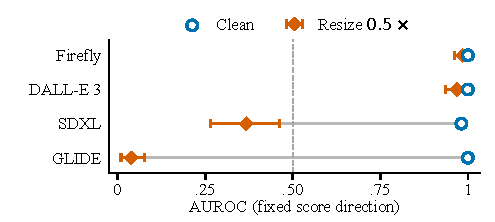
\includegraphics[width=\linewidth]{generator_sensitivity.pdf}
\caption{Half-size resizing, with 100 real and 50 synthetic images per generator. Bars show pointwise 95\% source-stratified bootstrap intervals. The dashed line marks chance; score direction is unchanged.}
\label{fig:generators}
\end{figure}

\begin{samepage}
\noindent\textbf{Comparison with the authors' implementation.}
Using identical weights, we compare our FFT-based extraction with the unmodified authors' code on 25 originals under the seven tabulated conditions.
All 175 detection decisions and source predictions agree, as do matched task metrics; the largest absolute $z$ difference is $3.54\times10^{-7}$.
On the RTX 2060, median runtime falls from 44.8 to 2.94 seconds, with a median paired speedup of $15.1\times$.
Peak logical allocation falls from 10.76 to 0.81\,GiB, although this does not measure physical VRAM residency.
Acceleration reduces offline evaluation cost but does not improve robustness.
\par
\end{samepage}

\noindent\textbf{Practical implications.}
Calibration on processed real images may recover detection rates when ranking remains strong, but cannot repair ranking reversals.
Native-resolution features or aggregation across crops deserve investigation, although they may change feature distributions and increase computation.
These possibilities remain untested.
Larger, content-disjoint tests with actual platform outputs would strengthen the study: our processing is simulated, source resolution and encoding differ, and overlap with checkpoint training data is unknown.
The small upstream comparison supports implementation agreement rather than broad robustness.
